\documentclass{article}
\usepackage{tikz}
\usetikzlibrary{positioning}

\begin{document}

\begin{figure}[h]
    \centering
    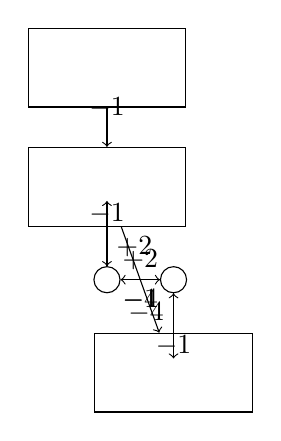
\begin{tikzpicture}[node distance=0.5cm, auto]
        % Define nodes
        \node (n1) [draw, circle] {};
        \node (n2) [draw, circle, right=of n1] {};
        
        % Draw edges with labels
        \path[->] (n1) edge node {$+2$} (n2);
        \path[->] (n2) edge node {$-4$} (n1);
        \path[->] (n1) edge node [above] {$-1$} ++(0,1);
        \path[->] (n2) edge node [below] {$-1$} ++(0,-1);
        
        % Draw the 3-line graph
        \node [draw, rectangle, minimum width=2cm, minimum height=1cm, above=of n1] (line1) {};
        \node [draw, rectangle, minimum width=2cm, minimum height=1cm, below=of n2] (line2) {};
        \node [draw, rectangle, minimum width=2cm, minimum height=1cm, above=of line1] (line3) {};
        
        % Connect the lines
        \path[->] (line1) edge node {$+2$} (n1);
        \path[->] (line2) edge node {$-4$} (n2);
        \path[->] (line3) edge node [above] {$-1$} (line1);
        \path[->] (line1) edge node [below] {$-1$} (line2);
    \end{tikzpicture}
    
    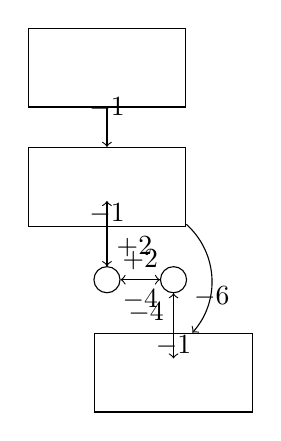
\begin{tikzpicture}[node distance=0.5cm, auto]
        % Define nodes
        \node (n1) [draw, circle] {};
        \node (n2) [draw, circle, right=of n1] {};
        
        % Draw edges with labels
        \path[->] (n1) edge node {$+2$} (n2);
        \path[->] (n2) edge node {$-4$} (n1);
        \path[->] (n1) edge node [above] {$-1$} ++(0,1);
        \path[->] (n2) edge node [below] {$-1$} ++(0,-1);
        
        % Draw the 3-line graph with modified twist
        \node [draw, rectangle, minimum width=2cm, minimum height=1cm, above=of n1] (line1) {};
        \node [draw, rectangle, minimum width=2cm, minimum height=1cm, below=of n2] (line2) {};
        \node [draw, rectangle, minimum width=2cm, minimum height=1cm, above=of line1] (line3) {};
        
        % Connect the lines with modified twist
        \path[->] (line1) edge node {$+2$} (n1);
        \path[->] (line2) edge node {$-4$} (n2);
        \path[->] (line3) edge node [above] {$-1$} (line1);
        \path[->] (line1) edge[bend left=45] node [below] {$-6$} (line2);
    \end{tikzpicture}
\end{figure}

\end{document}